\documentclass[uplatex,dvipdfmx,a4j,12pt]{jsarticle}

\usepackage[utf8]{inputenc}
\usepackage{graphicx}
\usepackage{amsmath}
\usepackage{comment}
\usepackage{color}
\usepackage{url}
\usepackage{siunitx}
\usepackage[version=4]{mhchem}
\usepackage{paralist}
\usepackage{longtable}
\usepackage{multirow}
\usepackage[dvipdfmx]{hyperref}
\usepackage{pxjahyper}
% \usepackage{makecell} % Add makecell package

\usepackage{enumitem}
\setlist[description]{parsep=5pt}
\setlist[enumerate]{parsep=5pt}

% コマンド定義
\newcommand{\divergence}{\mathrm{div}\,}  %ダイバージェンス
\newcommand{\grad}{\mathrm{grad}\,}  %グラディエント
\newcommand{\rot}{\mathrm{rot}\,}  %ローテーション
\newcommand{\diff}{\mathrm{d}} % 微分
\newcommand{\e}{\mathbf{e}} % 単位ベクトル


% 半角文字のパーセント、より右側は、コメントとして扱われます。

% タイトルページの内容をここで記述します。
\title{
  物理学実験IIレポート\\    % \\ は、強制的に改行するコマンドです。
  課題5 「電磁波の伝搬特性」
  }
\author{
  実験回: 第x回 \\
  氏名: \\
  実験者番号:
  \\
  共同実験者:
  }
\date{
  実験日:2025年 x月 x日~ x月 x日 \\
  提出日:2025年 x月 x日}  % 実験日と、提出日を記入して下さい

% ここから本文が始まります。
\begin{document}

% 上で設定したタイトルページの情報は、\maketitle があって始めて、コンパイル後に表示されます。
\maketitle

% レポートのフィードバックのコメントを希望しない場合には、
% 48行目から55行目までをコメントアウト(行頭に%を入れる)。
% コメントを希望する場合は、何について聞きたいかを具体的に書いて下さい。

% 縦方向の空白を挿入するコマンドです。em は行の高さ分、を意味する単位です。
\vspace{2em}
\begin{center}
    \begin{minipage}{0.5\linewidth}
        レポートのコメントを希望します。

        具体的には、○○について評価を下さい。
    \end{minipage}
\end{center}

\vspace{5em}  


% 概要は論文・レポート全体を一つの段落にまとめたものです。
% 物理の分野では、概要では段落分けをしません。
%
\begin{abstract}
    \textcolor{red}{このテンプレートにある指示文章は全て削除し、自分で書いた文章に差し替えること。残っていた場合は読みやすさを損ねるため減点とする。}
    (概要ではレポートの概要を簡潔に記述せよ。例えば、以下のようなものである。)
    ○○の目的のために、■■の実験を行った。
    その結果△△であることが確かめられた。
\end{abstract}

% 強制的に改ページを行う
\newpage


\section{目的}
% この実験のねらいが何であるかを、教科書の$\S2$を参考に簡潔にまとめる。
高周波回路は現代の通信技術において重要な役割を果たすだけでなく, より高精度な実験・測定を行うための基礎技術でもある.
本実験では, 高周波領域で現れる電磁波の波動性に着目してその伝播特性を調べると共に, 素子のインピーダンスやそれに起因する信号の反射を調べることを目的とする.

\section{原理}
% この実験に関連する原理を、教科書の$\S2$を参考に簡潔に記述する。
\subsection{電磁波}
電磁波は、電場と磁場が互いに直交しながら進行する波動である.

Maxwellの方程式から, 真空中の電磁波に対する波動方程式は次のように表される:
\begin{equation}
    \nabla^2 \mathbf{E} - \frac{1}{c^2} \frac{\partial^2 \mathbf{E}}{\partial t^2} = 0
\end{equation}
ここで、$\mathbf{E}$は電場ベクトル, $c = 1/\sqrt{\epsilon\varepsilon}$は光速である.
したがって, $x$方向に進行する電磁波は次のように表される:
\begin{equation}
    \mathbf{E}(x,t) = \mathbf{E_0} \exp{[i(\omega t - kx)]}
\end{equation}
ここで、$\mathbf{E_0}$は電場ベクトルの振幅, $k$は波数, $\omega$は角周波数である.
磁場の波 (磁波) についても同様の式が成り立つ.

より一般の誘電率$\varepsilon$と透磁率$\mu$を持つ媒質中での伝播を考えると, 電磁波は次式で表される:
\begin{equation}
  \mathbf{E}_x = \mathbf{E_0}\exp{(-\alpha z)} \exp{[i(\omega t - \beta z)]}
\end{equation}
ここで, 
\begin{gather}
  \alpha = \sqrt{\frac{\omega^2 \mu \varepsilon}{2} \left(\sqrt{1 + \frac{\sigma^2}{\omega^2 \varepsilon^2}} - 1\right)}, \\
  \beta = \sqrt{\frac{\omega^2 \mu \varepsilon}{2} \left(\sqrt{1 + \frac{\sigma^2}{\omega^2 \varepsilon^2}} + 1\right)},
\end{gather}
であり, $\sigma$は導電率である.

一般に$\sigma$は十分大きいと仮定できるので, $\alpha$は次のように近似できる:
\begin{equation}
  \alpha \approx \sqrt{\frac{\omega^2 \mu \varepsilon}{2} \frac{\sigma}{\omega \varepsilon}} = \sqrt{\frac{\omega \mu}{2 \rho}}
\end{equation}
ここで, $\rho = 1 / \sigma$は導体の抵抗率である.
したがって, 電磁波が媒質に侵入できる深さ (表皮深さ) $\delta$は次のように表される:
\begin{equation}
  \delta = \frac{1}{\alpha} = \sqrt{\frac{2 \rho}{\omega \mu}}.
\end{equation}

\enskip

次に, 伝送経路中を伝播する電磁波について述べる.
ここでは平行導線 (レッヘル線) や同軸ケーブルといった, 比較的簡単で等価回路を用いて議論できる系について考える.

レッヘル線を模した平行導線とその等価回路の模式図を図\ref{fig:lecher_line}に示す.
\begin{figure}[h]
    \centering
    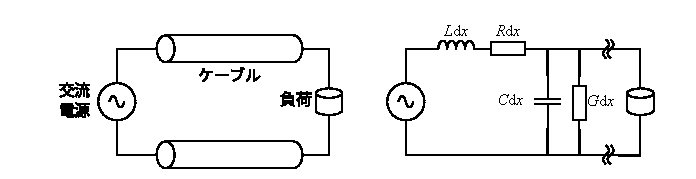
\includegraphics[width=0.9\linewidth]{img/lecher_line.pdf}
    \caption{平行導線とその等価回路}
    \label{fig:lecher_line}
\end{figure}

等価回路に示したように, 平行導線には単位長さあたりの抵抗$R$のほかに, 単位長さあたりのインダクタンス$L$, 
2つの導線間の静電容量$C$, コンダクタンス$G$が存在する.
このとき, 直列インピーダンス$Z$は$Z = R + i\omega L$, 並アドミニスタンス$Y$は$Y = G + i\omega C$と表される.
微小長さ$\diff z$間で生じる電位差$\diff V$と, 電流の変化$\diff I$は次のように表される:
\begin{equation}
  \frac{\diff V}{\diff x} = - Z I, \quad \frac{\diff I}{\diff x} = - Y V.
\end{equation}
ここから, 導線の特性インピーダンス$Z_0$を求めると,
\begin{equation}
  Z_0 = \frac{V}{I} = \sqrt{\frac{Z}{Y}} 
\end{equation}
一般に高周波伝達線路での損失は小さいことから, $R \ll 1$, $G \ll 1$と仮定できる.
したがって, $Z_0$は次のように近似できる:
\begin{equation}
  Z_0 \approx \sqrt{\frac{i\omega L}{i\omega C}} = \sqrt{\frac{L}{C}}.
\end{equation}
また, このとき伝達経路中の伝送速度として,
\begin{equation}
  v = \frac{1}{\sqrt{LC}}
\end{equation}
が成り立つ.

\enskip

同軸ケーブルにおいては, 単位長さあたりのインダクタンス$L$, 単位長さあたりの静電容量$C$は次のように表される:
\begin{equation}
  L = \frac{\mu_0}{2\pi} \ln\left(D/d\right), \quad C = \frac{2\pi\varepsilon_r \varepsilon_0}{\ln\left(D/d\right) }
\end{equation}
ここで, $D$は同軸ケーブルの外径, $d$は内径, $\varepsilon_r$は外部導体と中心導体の間の比誘電率である.

したがって, 同軸ケーブル中の伝送速度は次のように表される:
\begin{equation}
  v = \frac{1}{\sqrt{LC}} = \frac{c}{\sqrt{\varepsilon}}
\end{equation}

\enskip

また, 電磁波の特徴的な性質として, 異なる媒質へ入射したときの反射と透過がある.

媒質1から媒質2へ入射したとき, 反射率$\Gamma$と透過率$T$は次のように表される:
\begin{align}
  \Gamma &= \frac{Z_2 - Z_1}{Z_2 + Z_1}, \label{eq:reflection}\\
  T &= \frac{2Z_1}{Z_2 + Z_1}
\end{align}
ここで, $Z_1$は媒質1のインピーダンス, $Z_2$は媒質2のインピーダンスである.
このことから,2媒質のインピーダンスが異なるときには,必ず反射が生じることが分かる.

この結果として,信号線の末端に負荷を接続した場合においても,負荷のインピーダンスが信号線のインピーダンスと異なるときには反射が生じる.
入力側のインピーダンスを$Z_0$,負荷のインピーダンスを$Z_L$とするとき,反射係数$\Gamma$は次のように式\eqref{eq:reflection}と同じ表式で表される:
\begin{equation}
  \Gamma = \frac{Z_L - Z_0}{Z_L + Z_0} \label{eq:reflection_2}
\end{equation}

抵抗器のインピーダンスは抵抗値と等しいことから,末端を開放した際には$Z_L = \infty$,$\Gamma = 1$,短絡した際には$Z_L = 0$,$\Gamma = -1$となる.
また,負荷のインピーダンスが信号線のインピーダンスと等しい場合には,$\Gamma = 0$となり,反射は生じない.

負荷としてコイルやコンデンサを接続した場合には,そのインピーダンスは周波数に依存した複素数となることから,周波数に応じて位相差$\sigma$が変化する.
式\eqref{eq:reflection_2}から, 
\begin{alignat}{4}
  &\text{コイル}\quad & Z_L &= i\omega L, & |\Gamma| &= 1, & \delta &= 2\arctan\left(\frac{ Z_0}{ \omega L}\right) \\
  &\text{コンデンサ}\quad & Z_L &= \frac{1}{i\omega C},\, & |\Gamma| &= 1,\, & \delta &= -2\arctan\left({Z_0\omega C}\right)
\end{alignat}
となることわかる.

次に,$Z_L$の負荷が線路の途中に接続されている場合について考える.
この場合には,反射率は次のように表される:
\begin{equation}
  \Gamma = -\frac{Z_0}{2Z_L + Z_0}
\end{equation}
また,負荷の先の線路への透過率については,
\begin{equation}
  T = \frac{2Z_L}{2Z_L + Z_0}
\end{equation}
となる.すなわち,負荷がない場合$Z_L = \infty$では 反射率$\Gamma =  0$, 透過率$T = 1$となるが,負荷がある場合には透過率は1よりも小さくなることがわかる.


\subsection{共振回路}
回路の大きさが波長に比べて十分小さい集中定数回路においては,コイルやコンデンサを組み合わせることで共振回路を構成することができる.

$LRC$直列回路においては,回路のインピーダンス$Z$が,
\begin{equation}
  Z = R + i\omega L - \frac{i}{\omega C}, |Z| = \sqrt{R^2 + \left(\omega L - \frac{1}{\omega C}\right)^2}
\end{equation}
であることから,$\omega_0 L = 1/\omega_0 C$のとき,$|Z|$が最小となり,系に流れる電流は最大となる.
この現象を共振と呼び,その周波数 (共振周波数) を$f_0$とすると,
\begin{equation}
  f_0 = \frac{\omega_0}{2\pi} = \frac{1}{2\pi\sqrt{LC}}.
\end{equation}
となる.

回路の大きさが波長に比べて無視できないほど大きい場合には,分布定数回路と呼ばれる回路を考えることができる.

例えば,長さ$d$の伝送線路の先に反射率$\Gamma$の負荷を接続した場合,距離$d$間での位相変化を無視できないことから,入力側からみた回路の特性インピーダンスは,
\begin{equation}
  Z_d = \frac{1+\Gamma \exp{(-2ikd)}}{1-\Gamma \exp{(-2ikd)}}Z_0
\end{equation}
と表され,$\Gamma$が正の実数であるとき,$|Z_d|$が最小となるのは,
\begin{equation}
  d = (2n + 1)\frac{\lambda}{4}, \quad (n = 0, 1, 2, \cdots)
\end{equation}
となるときである.
これは自由端-固定端の共鳴と同じである.

\subsection{ヘテロダイン検波}
高周波 (搬送波) を別の周波数の信号と混合することで,情報を伝達することができる.
混合の手法には,搬送波の振幅を変化させる振幅変調 (AM),搬送波の周波数や位相を変化させる周波数変調 (FM)や位相変調がある

ヘテロダイン検波とは,搬送波と信号を混合することで,信号の周波数を変化させる手法である.
本実験ではダブルバランスドミキサ (DBM) を用いて,周波数混合を行った.
周波数$f$, 位相$\delta$の高周波信号をDBMのRF端子へ入力し,LO端子には高周波信号と僅かに異なる周波数$f_L$の高精度局所信号を入力することで,IF端子には信号の積として,
\begin{align}
  E_\mathrm{IF} &\propto E_\mathrm{RF} E_\mathrm{LO} \nonumber \\
  &\propto \cos\left(2\pi f t + \delta\right) \cos\left(2\pi f_L t\right) \nonumber \\
  &\propto \cos\left(2\pi (f + f_L) t + \delta\right) + \cos\left(2\pi (f - f_L) t + \delta\right)
\end{align}
なる,高周波成分$f + f_L$と低周波成分$f - f_L$の混ざった信号が得られる.
この信号をローパスフィルタで低周波成分 (中間周波数) のみを取り出すことで,高周波信号の振幅に比例し, 位相情報を含む信号 (ダウンコンバート信号)を得ることができる.

\subsection{ダイポールアンテナ}
電流が時間的に変化する導体の周りには, 電場と磁場が発生する.
また逆に, 電場と磁場の時間変化によって電流が生じる.
これを利用して, 電磁波を放射・受信する素子をアンテナと呼ぶ.
ここでは, 図\ref{fig:dipole_antenna}ダイポールアンテナについて考える.

ダイポールアンテナの電流分布は次のように表される:
\begin{equation}
    I(x) = I_0 \left(1 - \frac{|z|}{d}\right)\sin\left(\omega t\right)
\end{equation}
ここで, $\omega$は印加する交流電源の角周波数である.
このとき, 保存の式から電荷密度について次のように表される:
\begin{equation}
  \frac{\partial \rho}{\partial t}  = - \frac{\partial I}{\partial z} = \pm \frac{I_0}{d}\sin\left(\omega t\right)
\end{equation}
したがって, 
\begin{equation}
  \rho = \mp \frac{I_0}{\omega d}\cos\left(\omega t\right)
\end{equation}

このとき, 双極子モーメント$\mathbf{p}$は次のように表される:
\begin{equation}
  \mathbf{p} = \int \rho \mathbf{r} dV = \mp \frac{I_0}{\omega d}\int \cos\left(\omega t\right) \mathbf{r} dV
  = -\frac{I_0 d}{\omega}\cos\left(\omega t\right) \mathbf{e}_\mathrm{z}.
\end{equation}

ここで, 双極子から十分離れた点$\mathbf{r}$でのポインティングベクトル$\mathbf{S}$は次のように表される:
\begin{equation}
  \mathbf{S} = \frac{1}{\mu_0}\left(\mathbf{E} \times \mathbf{H}\right) =
  \frac{\mu_0}{(4\pi)^2c} \frac{\ddot{p}(t)\sin^2\theta}{r^2}\mathbf{e}_\mathrm{r}
\end{equation}
ここで, $\theta$は位置$\mathbf{r}$と双極子$\mathbf{p}$のなす角度であり, $\mathbf{e}_\mathrm{r}$は位置ベクトルの単位ベクトルである.
したがって, 電磁波のエネルギー流束は次のように表される:
\begin{equation}
  \mathbf{S} = \frac{\mu_0}{(4\pi)^2c} \frac{\sin^2\theta}{r^2}(I_0 d \omega)^2 \cos^2\left(\omega t\right)\,\mathbf{e}_\mathrm{r}
\end{equation}
時間平均をとると,
\begin{equation}
  \langle \mathbf{S} \rangle = \frac{\mu_0}{(4\pi)^2c} \frac{\sin^2\theta}{r^2}(I_0 d \omega)^2 \frac{1}{2}\,\mathbf{e}_\mathrm{r}
\end{equation}
となる.

したがって, 距離$r$離れた点で受信するとき, 受信側で得られる電力$P$は次のように表される:
\begin{equation}
  P \propto |\langle \mathbf{S} \rangle| \propto \frac{\sin^2\theta}{r^2}
\end{equation}

\section{課題1: 高周波信号測定の基礎}
\subsection{オシロスコープによる測定}
\subsubsection{方法}
% 方法について簡潔に記述する。
% 必要に応じて回路図や実験装置の配置を挿入する。テキストに記載された図と等価な場合は、「テキスト図XXの回路を用いて...」のように引用してよい。
実験に用いた回路はテキスト図16 (p. 141) のように, ファンクションジェネレータで発生させた信号をパワーディバイダによって分割し, 1 [m]の同軸ケーブルを介して, オシロスコープに接続させた.

このとき, まず初めにオシロスコープで測定された信号振幅からパワーディバイダが信号を均等に分割できていることを確かめた.
ただし, 測定のしやすさから, 以降断りのない限りはPeak to Peak (PP) 値を用いる.

そのうえで, オシロスコープのCh.2の入力カップリングをDC 50 \si{\ohm}からDC 1M \si{\ohm}に変更し, Ch.1とCh.2の信号波形を比較した.
また, Ch.2に50 [\si{\ohm}] の貫通ターミネータを接続し, 信号波形の変化を観察した.

次に, Ch.2の入力カップリングをDC 50\si{\ohm}に戻した上で,ファンクションジェネレータの出力部分に6 dBの減衰器を接続し, Ch.1とCh.2の信号波形を比較するとともに, 信号の減衰を測定した.
さらに, Ch.2に接続する同軸ケーブルの長さを10 [m]に変更し, Ch.1とCh.2の信号の位相差 (立上りの時間差) を測定し, これによって信号の伝達速度を求めた.



\subsubsection{結果}
% 実験で得た結果を記す。
% 例えば、実験データの表、グラフなどを記載し、それらについて文章で説明する。
入力カップリング50\si{\ohm}においてCh.1とCh.2の信号波形を比較した結果のCh.1, Ch.2の信号振幅を表\ref{table:1-1-1}に示す.
\begin{table}[h]
    \centering
    \caption{オシロスコープのCh.1, Ch.2の信号振幅.}
    \label{table:1-1-1}
    \begin{tabular}{cc}
        \hline
        & 信号振幅 [mV]\\
        \hline\hline
        Ch.1 & 920  \\
        Ch.2 & 860  \\
        \hline
    \end{tabular}
\end{table}
Ch.1の信号振幅は920 [mV], Ch.2の信号振幅は860 [mV]であり, 2つの信号はほぼ同じ振幅であることがわかる.

次に, Ch.2の入力カップリングをDC 1M \si{\ohm}に変更した場合の信号波形を比較した結果のCh.1, Ch.2の信号振幅を表\ref{table:-1-1-2}に示す.
\begin{table}[h]
    \centering
    \caption{入力カップリングをDC 1M \si{\ohm}に設定したときのオシロスコープのCh.1, Ch.2の信号振幅.}
    \label{table:-1-1-2}
    \begin{tabular}{ccc}
        \hline
        & 信号振幅 [V] & 貫通ターミネータ接続後 [mV]\\ % Use \makecell for line break
        \hline\hline
        Ch.1 & 1.35 & 920 \\
        Ch.2 & 1.76 & 890\\
        \hline
    \end{tabular}
\end{table}
図に示したように, 入力カップリングをDC 1M \si{\ohm}に変更することで, 観測された信号振幅の増大が確認できた.
また図\ref{table:-1-1-2}に示すように, 貫通ターミネータを接続した場合の信号振幅はCh.1が920 [mV], Ch.2が890 [mV]であり, いずれも元の状態に戻ったことがわかる.

次に, Ch.2の入力カップリングをDC 50\si{\ohm}に戻した上で,ファンクションジェネレータの出力部分に6 dBの減衰器を接続し, Ch.1とCh.2の信号波形を比較した結果のCh.1, Ch.2の信号振幅を表\ref{table:1-1-3}に示す.
\begin{table}[h]
    \centering
    \caption{オシロスコープのCh.1, Ch.2の信号振幅.}
    \label{table:1-1-3}
    \begin{tabular}{ccc}
        \hline
        & 信号振幅 [mV]& 減衰率[dB]\\
        \hline\hline
        Ch.1 & 468 & 5.87\\
        Ch.2 & 437 & 5.88\\
        \hline
    \end{tabular}
\end{table}
Ch.1の信号振幅は468 [mV], Ch.2の信号振幅は437 [mV]であり, 最初の状態からの減衰率はdBで表すとそれぞれ5.87 [dB], 5.88 [dB]であった.
これは, 減衰器の減衰率が6 [dB]であることから, 減衰器の設計値とほぼ一致していることがわかる.

最後に, Ch.2に接続する同軸ケーブルの長さを10 [m]に変更し, Ch.1とCh.2の信号の位相差を測定した結果, $\Delta t = 45.6$ [ns]であった.
このとき, 信号中を伝達する電磁波の伝達速度$c_\mathrm{cable}$は,
\begin{equation}
  c_\mathrm{cable} = \frac{L}{\Delta t} = \frac{9\,\mathrm{[m]}}{45.6 \times 10^{-9}\,\mathrm{[s]}} \approx 2.0 \times 10^8 \mathrm{\,[m/s]}
\end{equation}

と求まる.







\subsubsection{考察}
% テキストに記載された考察事項に沿った考察を記入する。
% 上記に加えて、独自の視点での考察も記すことを推奨する。


原理の節の式\ref{geasfdlkfsdfafdkasdjfklfdajlkfj} に示したように,誘電体中における光速は真空中の光速$c$よりも遅くなる.
したがって, 測定された伝達速度$c_\mathrm{cable}$から, 同軸ケーブルの誘電率$\varepsilon_\mathrm{cable}$を求めることができる:
\begin{equation}
  \varepsilon_\mathrm{cable} = \left(\frac{c}{c_\mathrm{cable}}\right)^2 \approx \left(\frac{3.0 \times 10^8\,\mathrm{[m/s]}}{2.0 \times 10^8\,\mathrm{[m/s]}}\right)^2 \approx 2.3
\end{equation}
これは, 同軸ケーブルによく用いられる誘電体であるポリエチレンの誘電率$\varepsilon_\mathrm{PE} \approx 2.3$とよく一致していることが分かる.



\subsection{オシロスコープによる測定}
\subsubsection{方法}
まず始めに,同軸ケーブルにおよる信号の減衰を測定するために,テキスト図17のように標準信号発生器からの信号をパワーディバイダで分割し,1 [m]と10 [m]の同軸ケーブルを介してパワーメータのA, B端子に接続した.
パワーメータでは,A端子の電力およびA, B端子の電力比を測定することができる.
標準信号発生器から出力 0 [dBm] の正弦波を発生させ,その周波数を変えることでA端子の信号電力とA, B端子の電力比の周波数依存性を測定した.

次に,テキスト図18のように1 [m] と10 [m] 同軸ケーブルを並列に接続することで信号の重ね合わせを行った.
このとき,先と同様に出力 0 [dBm] の正弦波を入力し,A端子で測定される電力とA, B端子の電力比の周波数依存性を測定した.

\subsubsection{結果}

\subsubsection{考察}

\subsection{パワーメータによる測定}
\subsubsection{方法}

\subsubsection{結果}

\subsubsection{考察}


\section{課題2: インピーダンス不整合による電磁波の反射}
\subsection{方法}

\subsection{結果}

\subsection{考察}


\section{課題3: 集中定数回路と分布定数回路における共振特性}
\subsection{方法}

\subsection{結果}

\subsection{考察}


\section{課題4: ヘテロダイン検波}
\subsection{方法}

\subsection{結果}

\subsection{考察}


\section{課題5: 半波長アンテナにおける電気双極子放射}
\subsection{方法}

\subsection{結果}

\subsection{考察}


\section{結論}
実験目的を要約して記述し、それに対応する結論を簡潔に記述すること。


% 参考にした文献があれば記述する。以下の例を書き換えること。
\begin{thebibliography}{9}

    \bibitem{bunken1}
        A. Einstein, B. Podolsky, and N. Rosen, 
        Phys. Rev. \textbf{47}, (1935) 777.
        % いわゆるEPRパラドックスと呼ばれる量子力学に関する論文

    \bibitem{bunnken2}
        J.J. Aubert \textit{et al.},
        Phys. Lett. B \textbf{123} (1983) 275.
        % いわゆるEMC効果と呼ばれる現象についての実験の論文
    
\end{thebibliography}

\end{document}
